\chapter{Descrição do Sistema ``Admins''}
\label{chap4}

Dado a escolha de um banco de dados em grafo como o Neo4j, enfrentamos o problema de ser complicado para pessoas ingênuas ao schema do banco de dados manipularem os itens de dados, além de ser pouco seguro gerenciá-los diretamente através de uma Cypher.Desta forma é possível facilmente realizar consultas muito pesadas, ou que tem consequências difíceis de reverter, de maneira acidental.

O sistema ``Admins'' foi desenvolvido com o objetivo de proporcionar uma interface amigável para mais facilmente gerenciar os dados, evitando os problemas mencionados acima. Através desse sistema os usuários podem criar, editar, conectar e desconectar arbitrariamente qualquer nó no grafo do banco de dados.

\section{Perfis e Listas}

Junto com o time de Design, identificamos uma maneira de entender e visualizar o grafo que está armazenado no banco, dando para cada nó uma página de perfil, que mostra e permite edição de suas propriedades e relações, além de uma página de lista/pesquisa para cada rótulo (relevante) no banco de dados. A partir deste isomorfismo, foi possível criar uma interface que permite aos usuários navegarem e editarem o grafo de maneira intuitiva.

\begin{figure}[H]
    \centering
    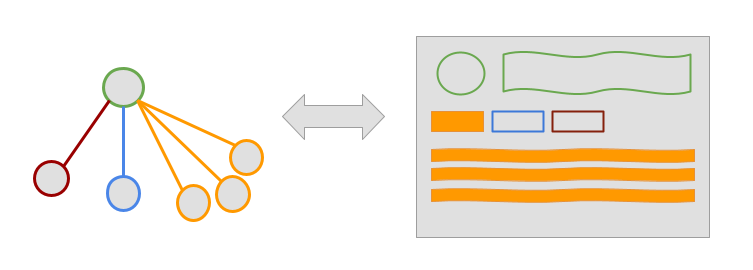
\includegraphics[width=1.0\linewidth]{Imagens/chap04/perfil-isomorfismo.png}
    \caption{Abstração de um \textbf{nó dono} (verde) está relacionado à \textbf{um nó de rótulo X} (vermelho), \textbf{um de rótulo Y} (azul), e possui relação com \textbf{três nós de rótulos Z} (amarelos) no grafo armazenado no banco de dados.}
    \label{fig:isomorphism}
\end{figure}

Temos então dois tipos de telas:
\begin{itemize}
    \item Perfis - Com as propriedades do nó dono na parte superior da tela, e diferentes abas (uma para cada tipo de relação que o nó possui) na parte inferior. Dentro de cada aba, uma lista de elementos com os nós vizinhos através daquele tipo de relação. Tal lista de elementos possui hiperlinks para páginas de perfis deste vizinhos. Desta maneira conseguimos andar pelo grafo através dos nós e relações, e em cada passo do caminho passamos pelo perfil do dó atual, com ações como edição, criação ou conexão entre nós.
        
    \begin{figure}[H]
        \centering
        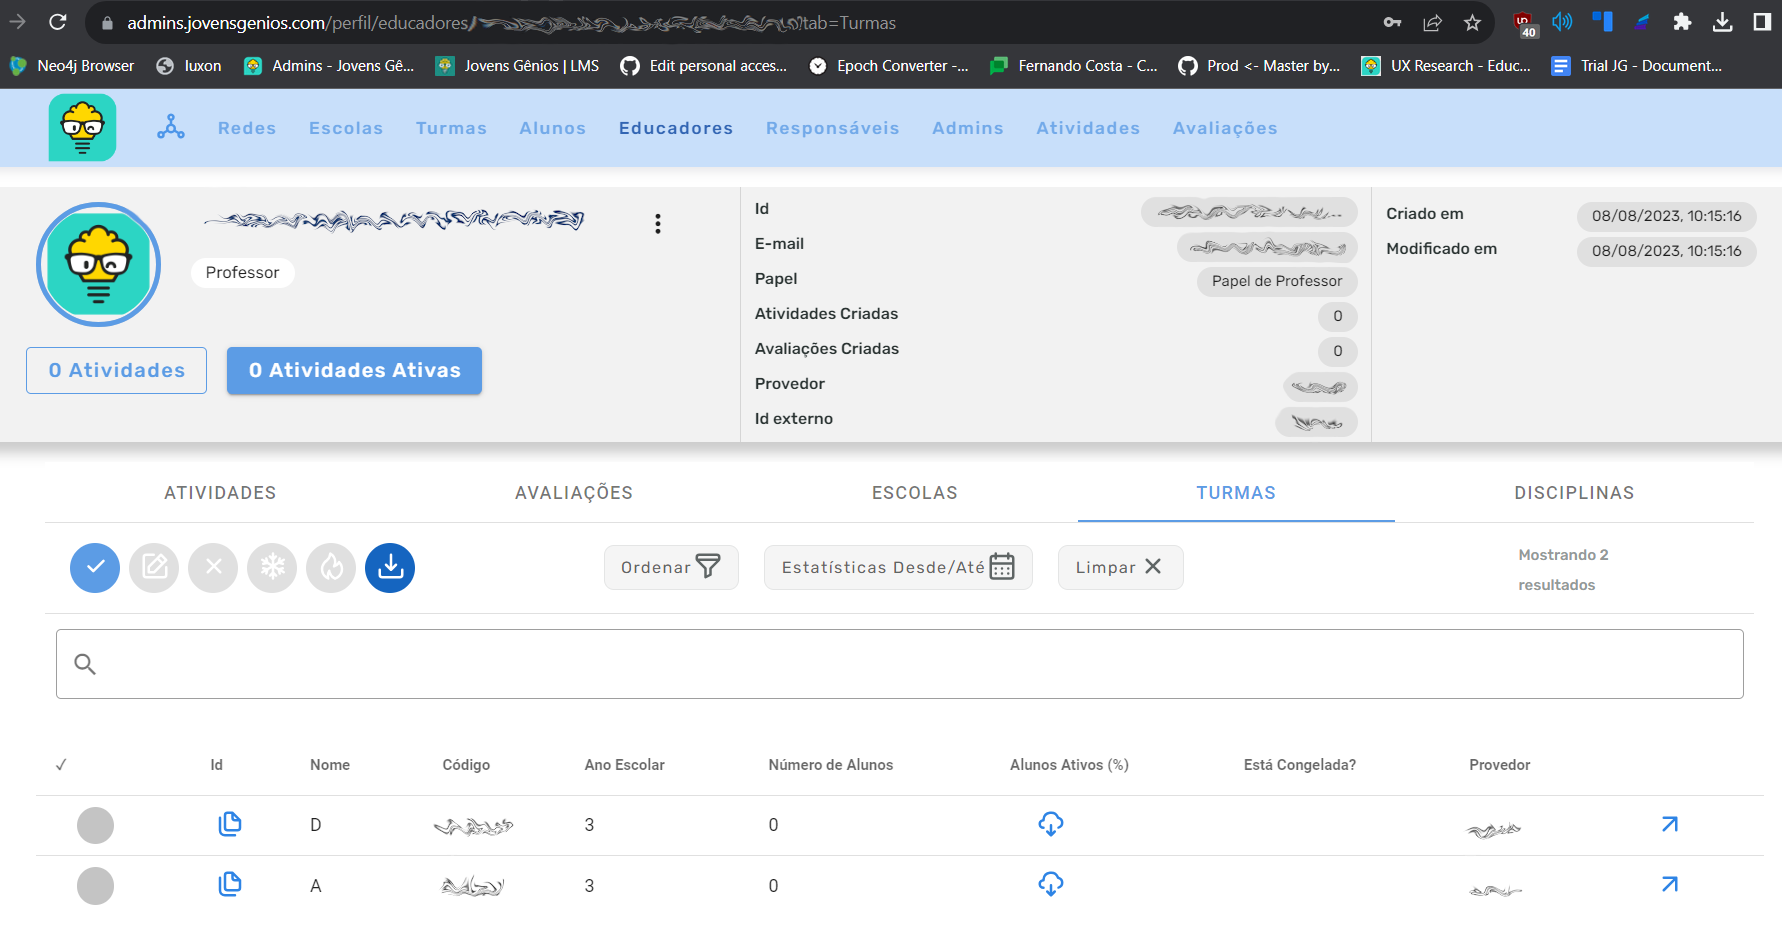
\includegraphics[width=1.0\linewidth]{Imagens/chap04/perfil-exemplo.png}
        \caption{Página de Perfil de um educador. Note as ações em azul ou cinza (dependente de selecionar um elemento para acessá-la) no cabeçalho da lista de vizinhos. Inclui edição, remoção e criação da aresta, entre o nó do perfil e os elementos selecionados, assim como outras ações específicas do \textit{tipo} da aba (Congelar/Descongelar turma).}
        \label{fig:profile-exemple}
    \end{figure}
    
    \item Listas - Precisamos começar a navegar pelo grafo a partir de algum nó inicial. Para isso existem as páginas de listas. Nelas são listados todos os elementos de um certo \textit{tipo} (de forma paginada), com hiperlinks para suas páginas de perfil. Também possui funcionalidades de busca e filtragem genéricas, além de acesso à ações diretas com os elementos listados.
\end{itemize}

A vantagem dessa modelagem é que conseguimos perceber que toda página de perfil (e de lista) segue a mesma regra, logo o código referente à sua implementação pode ser reutilizado. Ná prática, a aplicação consiste em apenas uma página de perfil e uma página de lista (além da página de login/autenticação), além de mapas que definem as especificidades de cada caso, facilitando sua manutenção e minimizando o tamanho do código, consequentemente minimizando também bugs em produção.

\section{Aplicação Cliente}

O objetivo da aplicação cliente (\textit{frontend}) é gerar uma interface que um usuário ingênuo consegue interagir, e, para cada ação realizada, gerar uma requisição em GraphQL que é enviada ao servidor (\textit{backend}). Utilizamos o framework web Vue.js para realizar a construção das páginas definidas acima.

O frontend então é composto pelas duas principais páginas do sistema, uma camada superior que controla os formulários e ações globais, e diversos componentes Vue específicos que são utilizados em ambas as páginas. Além disso possuímos diversos arquivos "úteis", que informam o que cada perfil de cada \textit{tipo} possui de específico, como por exemplo quais as ações específicas que são liberadas, dependendo do \textit{tipo} do perfil e do \textit{tipo} da aba.

\begin{figure}[H]
    \centering
    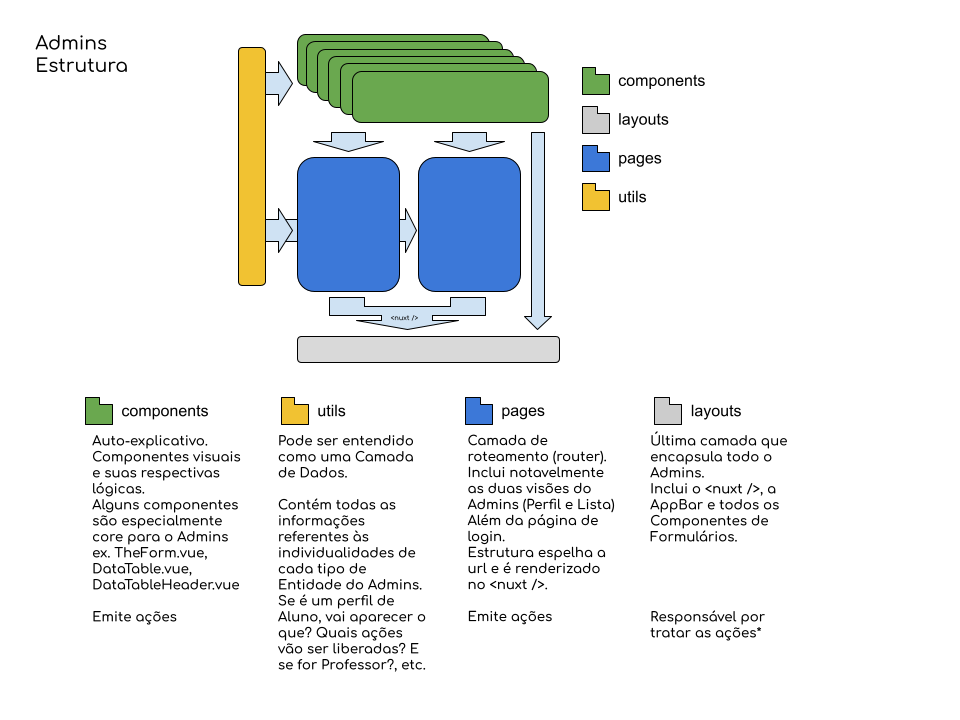
\includegraphics[width=1.0\linewidth]{Imagens/chap04/front-estrutura.png}
    \caption{Documentação criada para Jovens Gênios.}
    \label{fig:profile-exemple}
\end{figure}

\subsection{Uso da InstropectionQuery}

A IntrospectionQuery é uma requisição disponibilizada pela neo4j/graphql que pede ao servidor o schema de dados armazenado nele, além de quais são as consultas (queries) e mutações (mutations) permitidas pela API. Assim conseguimos não só conhecer todas as requisições possíveis, seus argumentos e tipos, como também todos os \textit{tipos} definidos nas definições de tipos e cada uma de suas propriedades. Utilizamos tais informações, por exemplo, quando abrimos um formulário de edição, utilizando a resposta para montar dinamicamente o formulário ou as tabelas nas quais os dados vão frequentar. Se acrescentarem mais uma propriedade na definição de tipos no backend, automaticamente o frontend vai mostrar um campo para esta, sem nenhum deploy ou alteração necessária.
(Preocupações de Segurança do instropection query)

Tal abordagem de construção dinâmica de formulários e perfis é interessante e foi utilizada durante alguns meses, porém percebemos que muitas vezes não queremos que o usuário desse gerenciador tenha acesso direto à edição de alguns dos atributos de alguns nós. Alguns atributos são pensados para serem populados automaticamente por outros fluxos e não esperado que editados manualmente, e outros simplesmente são dados utilizados “debaixo dos panos” - mostrar qualquer propriedade automaticamente no sistema ``Admins'' acabava confundindo os usuários.

Optamos então para uma abordagem híbrida, na qual recebemos no frontend quais são os atributos do \textit{tipo} referente na montagem dos formulários de criação e edição - porém os filtramos, mostrando apenas os que são editáveis, através de mapas em arquivos guardados no "utils". Esta abordagem híbrida também é utilizada nas colunas das tabelas das listas, e em quais as propriedades que aparecem no cabeçalho do perfil.

Abaixo um exemplo de um dos arquivos JSON do diretório "utils" que é usado para definir as propriedades à serem mostradas em cada cabeçalho de cada perfil, e como devem ser mostrados.
\begin{lstlisting}
{
  "Student": {
    "header": [
      "Id",
      "email",
      "schoolYear",
      "points",
      "keys",
      "trophies",
      "provider",
      "externalId"
    ],
    "chips": [],
    "rects": [
      {
        "prop": "questionsAnsweredCount",
        "extra": "Questoes Feitas",
        "color": "#5C9CE5"
      },
      {
        "prop": "correctQuestionsAnsweredCount",
        "extra": "Corretas",
        "color": "#5C9CE5"
      }
    ]
  },
...
\end{lstlisting}

o componente de busca e filtragem da página de listas também se beneficia do InstrospectionQuery, pois consegue, de forma automática, listar todas as possibilidades de uma certa propriedade ENUM em um seletor. Sabendo qual o tipo de cada propriedade conseguimos realizar um render de um componente de input adequado para o usuário interagir.

\subsection{Formulário reutilizável}

\begin{lstlisting}
<v-form>
  <v-row no-gutters justify="end">
    <v-col cols="12" class="px-2">
      <v-text-field disabled label="Id" v-model="Id" outlined>
      </v-text-field>
    </v-col>
    <v-col
      cols="12"
      class="px-2"
      v-for="(property, i) in properties.strings"
      :key="i"
    >
      <v-row no-gutters>
        <v-col>
          <v-text-field
            :label="`${
              non_null[i] ? translate(i) + ' *' : translate(i)
            }`"
            v-model="property.value"
            :disabled="property.disableInput"
            outlined
          />
        </v-col>
      </v-row>
    </v-col>
    <v-col
      cols="6"
      class="px-2"
      v-for="(enumProperty, j) in properties.enums"
      :key="j"
    >
      <v-select
        :label="`${non_null[j] ? translate(j) + ' *' : translate(j)}`"
        :items="enumValues[j]"
        item-text="name"
        item-value="name"
        v-model="enumProperty.value"
        outlined
        @input="checkEnumChanged(enumProperty)"
      >
        <template slot="selection" slot-scope="{ item }">
          {{ translate(item.name) }}
        </template>
        <template slot="item" slot-scope="{ item }">
          {{ translate(item.name) }}
        </template>
      </v-select>
    </v-col>
    <v-col
      cols="6"
      class="px-2"
      v-for="(property, k) in properties.numerics"
      :key="k"
    >
      <v-text-field
        :label="`${non_null[k] ? translate(k) + ' *' : translate(k)}`"
        type="number"
        v-model="property.value"
        outlined
      />
    </v-col>
    <v-col
      cols="12"
      class="px-2"
      v-for="(property, w) in properties.dateTimes"
      :key="w"
    >
      <date-time-picker
        :label="`${non_null[w] ? translate(w) + ' *' : translate(w)}`"
        :datetime="property.value"
        @onChange="changedDateTime($event, w)"
      />
    </v-col>
    
    <v-col
      cols="3"
      class="pb-2"
      v-for="(property, y) in properties.booleans"
      :key="y"
    >
      <v-switch
        class="mt-0"
        v-model="property.value"
        :label="`${non_null[y] ? translate(y) + ' *' : translate(y)}`"
      ></v-switch>
    </v-col>
  </v-row>
</v-form>
\end{lstlisting}

O objeto \textit{properties} é populado com as informações resultantes do IntrospectionQuery, passando por uma filtragem opcional definida no \textit{utils}.

Além das propriedades editáveis do \textit{tipo}, que possuem um componente de interação específico dependendo de seu tipo, o sistema Admins possui também algumas ações e regras de negócios personalizadas, que também são incluidas no formulário com a diretiva v-if com uma propriedade que define se tal ação específica deve estar ativa.

\begin{lstlisting}
    <v-col cols="12" v-if=" isCreateSchool">
      <courses-picker
        @changedCourses="changedCoursesSelected"
      ></courses-picker>
    </v-col>
    ...
    isCreateSchool() {
      return this.$route.params.type == "School" && this.add == true;
    }
\end{lstlisting}


\subsection{Ações}

As ações de manipulações de dados foram classificadas em três categorias:
\begin{itemize}
    \item Ações de Perfil - Em toda página de perfil de um nó, é possível abrir o formulário de ações diretas no nó dono. Inclue a deleção, edição de suas propriedades, e opcionalmente outras ações personalizadas
    \item Ações de Aba - Em cada aba dentro de um perfil, no cabeçalho de suas listas de elementos e com uma cor mais escura, existe botões de ações referentes à relações do nó dono com outros nós do \textit{tipo} referente à aba selecionada. Inclue a criação de um novo nó, já conectado ao dono, conectar o dono à um nó existente do \textit{tipo} da Aba, e opcionalmente outras ações personalizadas
    \item Ações de Elementos - Em cada aba dentro de um perfil, no cabeçalho de suas listas de elementos e com uma cor mais clara, é possível interagir com botões de ações referentes à elementos da lista selecionados. Inclue a edição do nó selecionado, e a desconexão dele(s) ào dono, além de opcionalmente outras ações personalizadas
\end{itemize}
Toda ação, independente da categoria, é propagada à camada Controle, carregando consigo um objeto com as informações que a definem. Nessa camada então, com acesso ao(s) \textit{tipo(s)} referente(s), seu(s) id(s), conseguimos escolher qual dos arquivos .gql que contém a requisição á ser enviada ao servidor deve ser utilizado na requisição.
\begin{figure}
    \centering
    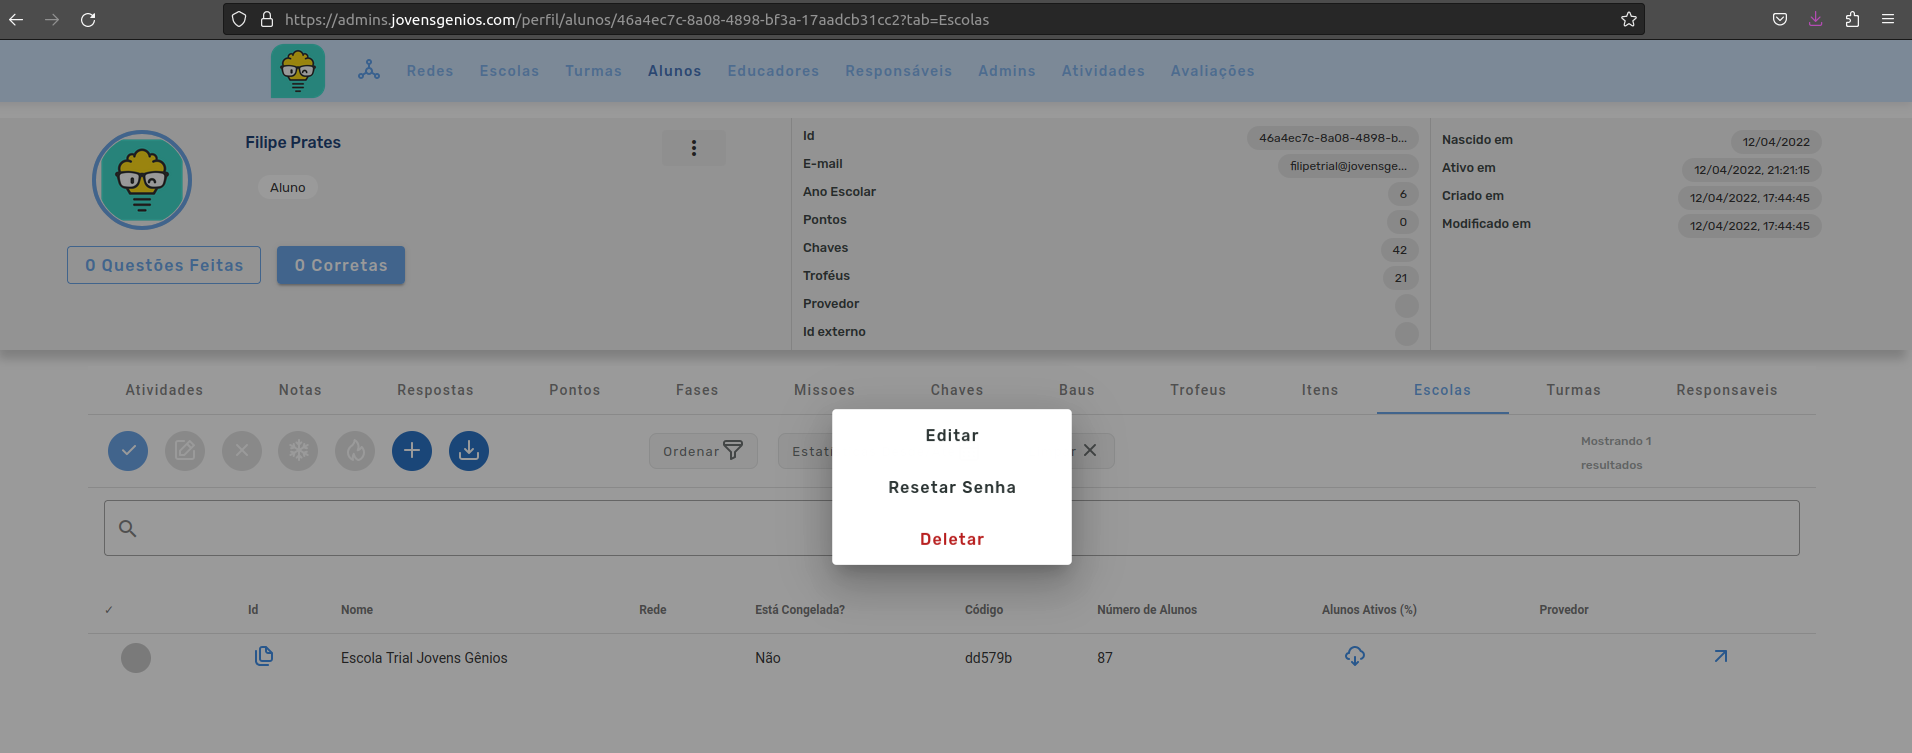
\includegraphics[width=1\linewidth]{Imagens/chap04/front-profile-actions.png}
    \caption{Interface das Ações de Perfil de um nó com \textit{tipo} Aluno}
    \label{fig:enter-label}
\end{figure}

\begin{figure}
    \centering
    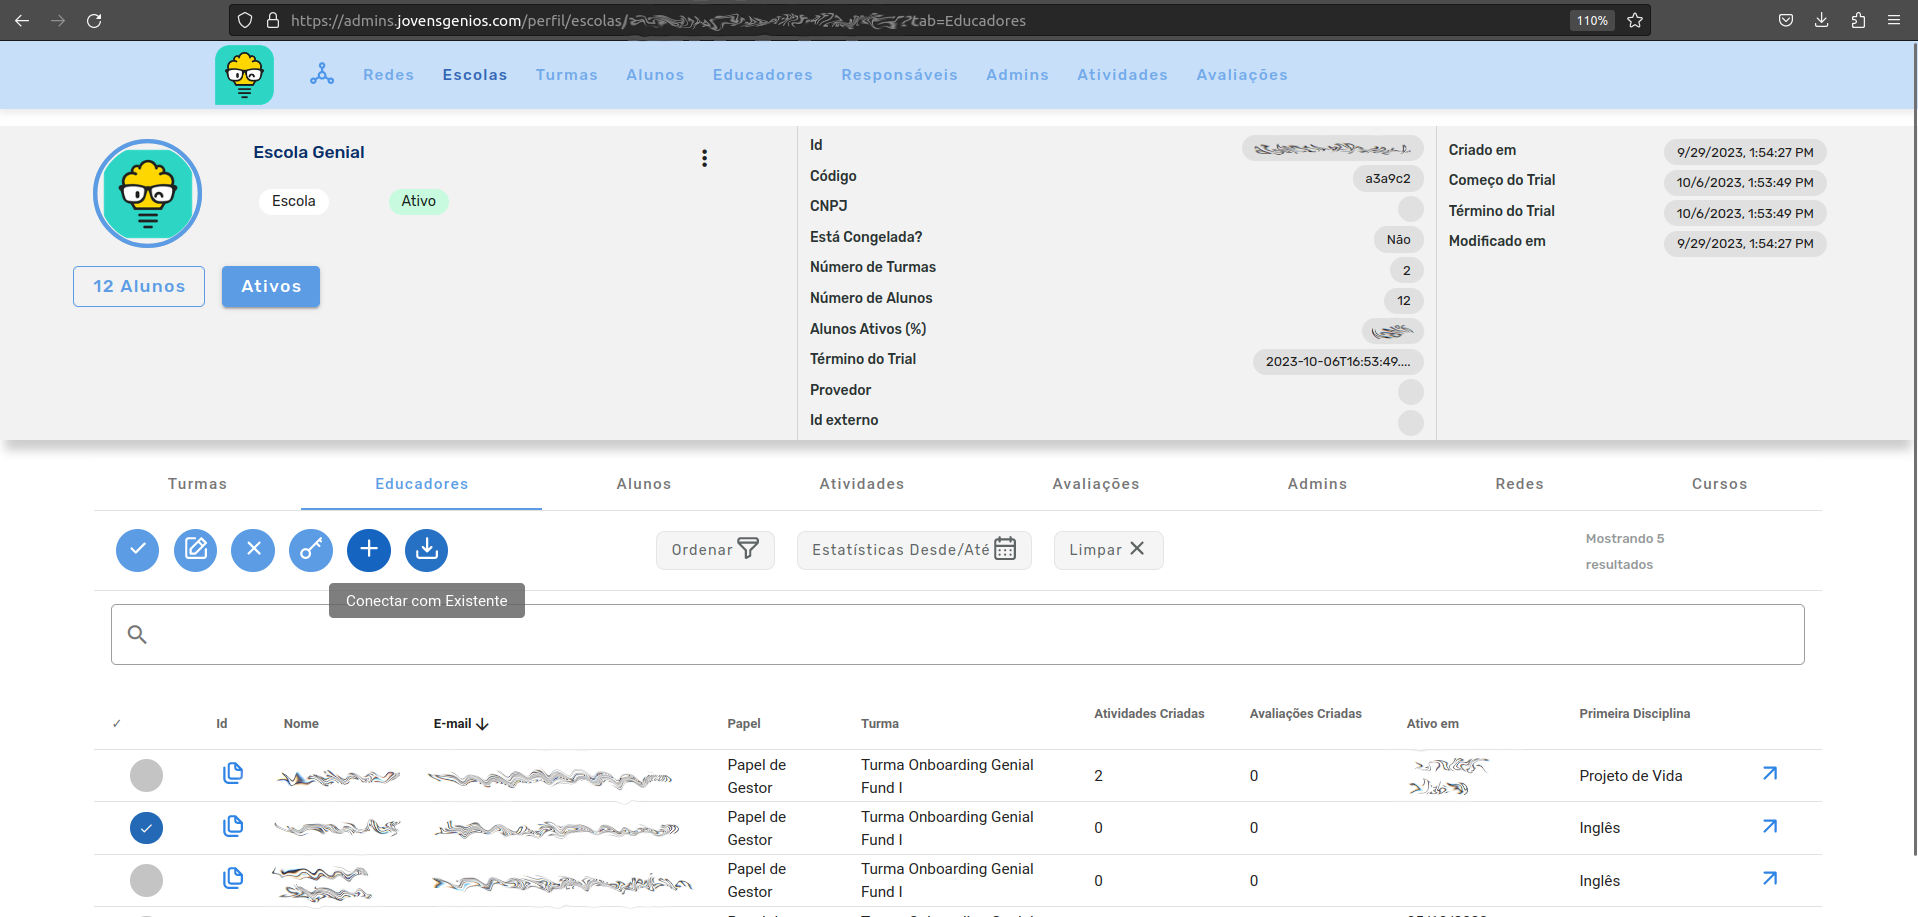
\includegraphics[width=1\linewidth]{Imagens/chap04/front-other-actions.png}
    \caption{Ações de Elementos e de Abas de um perfil do \textit{tipo} Escola, na Aba de relações com o \textit{tipo} Educadores.}
    \label{fig:enter-label}
\end{figure}

Abaixo um exemplo de função da camada de controle que lida com a ação de deletar múltiplos elementos selecionados de uma lista.

\begin{lstlisting}
async handleDelete(payload) {
  let type = "";
  for (let el of payload.elements) {
    if (confirm(`Certeza que quer deletar ${el.name}`)) {
        try {
          await this.$apollo.mutate({
            mutation: require(`@/graphql/${payload.type}/delete.gql`),
            variables: el,
          });
        } catch (e) {
          console.error(e);
          alert(e);
          return;
        }
      }
    }
  }
\end{lstlisting}

\section{Servidor com endpoint GraphQL}

O frontend, entretando, não se comunica diretamente com o banco de dados. A interface se comunica com uma camada intermediária através de requisições em GraphQL, e esta camada intermediária gera a Cypher resultante que então é executada no banco de dados. Nesta seção descreveremos como funciona o servidor responsável por este processo.

 \begin{figure}[H]

\begin{tikzpicture}[font=\small,thick]
 
% Start block
\node[draw,
    rounded rectangle,
    minimum width=2.5cm,
    minimum height=1cm] (block1) { Interface do ``Admins'' };
 
% Voltage and Current Measurement
\node[draw,
    below=0.8cm of block1,
    minimum width=2.5cm,
    minimum height=1cm
] (block2) { Servidor (Node.js) com endpoint GraphQL };
 
% Power and voltage variation
\node[draw,
    below=0.8cm of block2,
    minimum width=2.5cm,
    minimum height=1cm
] (block3) { Banco de Dados (Neo4j) };

\draw (block1) |- (block2);
\draw (block2) |- (block3);

\end{tikzpicture}
\caption{Fluxograma de comunicação entre partes do sistema }
\label{chap3:fluxograma}
\end{figure}

\subsection{Definições dos Tipos}

Uma das principais funções do servidor é a definição de cada \textit{tipo} existente no banco de dados. E nessa etapa, equivalente à definição das tabelas e campos num banco de dados SQL, que modelamos os dados do domínio e definimos cada \textit{tipo} de entidade que poderá ser manipulada através sistema gerenciador.

Como se tratam de muitos tipos diferentes, os separamos em diferentes arquivos para fim de organização, cada um com seu escopo. As definições de \textit{tipo} de cada arquivo respeitam um escopo definido, e possuem suas propriedades e tipos das propriedades, suas relações e tipos dos nós que são relacionados, além de definir aquelas Queries e Mutations que não são geradas automaticamente. Nestes arquivos, definimos também os tipos não nativos, como ENUMs específicos do escopo.

Os \textit{tipos} definidos geram as Labels que podem ser associadas aos nós do banco de dados.

Segue abaixo um exemplo simplificado de um arquivo de definição de tipos.
\begin{lstlisting}
"""
Battles types
"""
type Battle implements Context @node(labels: ["Battle", "Context"]) {
	id: ID @id
	name: String
	type: ContextType
	status: ContextStatus
	createdAt: DateTime! @timestamp(operations: [CREATE])
	updatedAt: DateTime! @timestamp(operations: [CREATE, UPDATE])
	assignedContext: [AssignedContext!]!
		@relationship(type: "OF_CONTEXT", direction: IN)
	studentAnswers: [StudentAnswer]
		@cypher(
			statement: """
			MATCH (this)<-[:OF_CONTEXT]-(:AssignedContext)<-[:OF_ASSIGNED_CONTEXT]-(sa:StudentAnswer) return distinct sa
			"""
		)
	topic: Topic @relationship(type: "SELECTED_IN_BATTLE", direction: OUT)
	task: Task @relationship(type: "BATTLE_IN_TASK_CONTEXT", direction: OUT)
	fromOrigin: BattleOrigin #TODO: Improve the property
	students: [AssignedContext]
		@cypher(
			statement: """
			MATCH (this)<-[:OF_CONTEXT]-(ac:AssignedContext)-[:ASSIGNED_TO]->(s:Student) return distinct ac
			"""
		)
	startsAt: DateTime
	endsAt: DateTime
	knowledgeArea: KnowledgeArea
		@relationship(type: "IN_KNOWLEDGE_AREA", direction: OUT)
}

enum StudentBattleStatus {
	NotStarted
	InProgress
	Finished
	Refused
}

type Query {
	botQuestionAnswerFraction(
		studentProgressInPlanet: Float
		questionDifficulty: Float
	): Float
}

type Mutation {
	mergeStudentsBattle(
		studentsIds: [ID!]
		battleId: ID!
		type: ContextType
	): [ID]
	setBattleResult(battleId: ID!): String
	deleteBattle(battleId: ID!): ID
	setChampionshipBattleResults(championshipId: ID!): String
}
\end{lstlisting}

\subsection{Mesclador de Definições de Tipos}
A biblioteca Neo4j/GraphQL espera apenas um arquivo de definição de tipos, então precisamos juntar todos eles utilizando expressões regulares e os padrões de cada arquivo de definição de tipo.

\begin{lstlisting}
const fs = require("fs");
const path = require("path");

let typeDefs = "";
let mutations = "";
let queries = "";
let subscriptions = "";
const dirname = path.join(__dirname, "./types/");

export const mergeTypeDefs = () => {
	const filenames = fs.readdirSync(dirname);

	filenames.forEach((filename) => {
		let content = fs.readFileSync(dirname + filename, "utf-8");

		concatMutations(content);
		concatQueries(content);
		concatSubscriptions(content);

		content = removeMutationsQueriesAndSubscriptions(content);
		typeDefs += content;
	});

	typeDefs += mergeMutationsQueriesAndSubscriptions(typeDefs);

	return typeDefs;
};

const concatMutations = (typeDef) => {
	const re = /(?<=Mutation\s*\{)(.*?[\s\S]*?)(?=\n\}\n|\r\n\}\r\n)/g;
	const mutationsInTypeDef = typeDef.match(re);

	if (mutationsInTypeDef && mutationsInTypeDef.length > 0) {
		mutations = mutations.concat(...mutationsInTypeDef);
	}
};

const concatQueries = (typeDef) => {
	const re = /(?<=Query\s*\{)(.*?[\s\S]*?)(?=\n\}\n|\r\n\}\r\n)/g;
	const queriesInTypeDef = typeDef.match(re);

	if (queriesInTypeDef && queriesInTypeDef.length > 0) {
		queries = queries.concat(...queriesInTypeDef);
	}
};

const concatSubscriptions = (typeDef) => {
	const re = /(?<=Subscription\s*\{)(.*?[\s\S]*?)(?=\n\}\n|\n\}\n|\r\n\}\r\n)/g;
	const subscriptionsInTypeDef = typeDef.match(re);

	if (subscriptionsInTypeDef && subscriptionsInTypeDef.length > 0) {
		subscriptions = subscriptions.concat(...subscriptionsInTypeDef);
	}
};

const removeMutationsQueriesAndSubscriptions = (typeDef) => {
	const reMutations = /type\s*Mutation\s*\{(.*?[\s\S]*?)(\n\}\n|\r\n\}\r\n)/g;
	const reQueries = /type\s*Query\s*\{(.*?[\s\S]*?)(\n\}\n|\r\n\}\r\n)/g;
	const reSubscriptions = /type\s*Subscription\s*\{(.*?[\s\S]*?)(\n\}\n|\r\n\}\r\n)/g;

	let newTypeDef = typeDef.replaceAll(reMutations, "");
	newTypeDef = newTypeDef.replaceAll(reQueries, "");
	newTypeDef = newTypeDef.replaceAll(reSubscriptions, "");
	return newTypeDef;
};

const mergeMutationsQueriesAndSubscriptions = (typeDef) => {
	if (mutations.length > 0) {
		typeDef += `\r\n\r\ntype Mutation {\r\n${mutations}\r\n}`;
	}
	if (queries.length > 0) {
		typeDef += `\r\n\r\ntype Query {\r\n${queries}\r\n}`;
	}
	if (subscriptions.length > 0) {
		typeDef += `\r\n\r\ntype Subscription {\r\n${subscriptions}\r\n}`;
	}

	return typeDef;
};
\end{lstlisting}

\subsection{Resolvers}

Aqui que tá a mágica 

\subsection{Geração do Schema para o banco de dados}

 Utilizamos a bibliotecas do driver da Neo4j para conectar ao banco, autenticando com usuário e senha.
 
 \begin{lstlisting}
import neo4j from "neo4j-driver";

const driver = neo4j.driver(
	process.env.NEO4J_URI || "bolt://localhost:7687",
	neo4j.auth.basic(
		process.env.NEO4J_USER || "neo4j",
		process.env.NEO4J_PASSWORD || "neo4j"
	),
	{
		maxConnectionLifetime: 8 * 60 * 1000,
		maxConnectionPoolSize: 50,
		connectionAcquisitionTimeout: 2 * 60 * 1000,
		disableLosslessIntegers: true,
	}
);
\end{lstlisting}

Então importamos os nossos resolvers e definições de tipos, e configuramos os plugins utilizados, como o Neo4jGraphQLAuthJWTPlugin, que permite a autenticação das requisições através de uma JWToken no campo de "Authorization" no header de cada requisição GraphQL.

 O Schema é então gerado instanciando um novo objeto Neo4jGraphQL() (da @neo4j/graphql), que recebe como argumentos o driver conectado ao banco de dados, as definições de \textit{tipos} mescladas, os resolvers e eventuais plugins.

\begin{lstlisting}
import { Neo4jGraphQL } from "@neo4j/graphql";
import { Neo4jGraphQLAuthJWTPlugin } from "@neo4j/graphql-plugin-auth";
const typeDefs = mergeTypeDefs();
async function initializeNeo4jGraphQL() {
	const neo4jGraphQL = new Neo4jGraphQL({
		driver,
		typeDefs: gql`
			${typeDefs}
		`,
		resolvers,
		plugins: {
			auth: new Neo4jGraphQLAuthJWTPlugin({
				secret: process.env.JWT_SECRET,
				algorithms: ["HS256"],
				credentialsRequired: false,
			}),
			config: {
				enableDebug: process.env.NODE_APP_ENV === "staging",
			},
		},
	});
	return await neo4jGraphQL.getSchema();
}
\end{lstlisting}

Em seguida o Apollo Server é inicializado com este Schema e o servidor express o publica nas portas definidas, aguardando as requisições.

\begin{lstlisting}
import { expressMiddleware } from "@apollo/server/express4";
    const app = express();
    app.use(cors());
    app.use(json({ limit: "20mb" }));
    app.use(express.urlencoded({ limit: "20mb", extended: true }));
    
	const apolloServer = new ApolloServer({
		schema: schema,
		introspection: true,  // Permite a requisição InstrospectionQuery
		playground: process.env.NODE_APP_ENV !== "production",
		plugins: [
			ApolloServerPluginLandingPageGraphQLPlayground(),
			{
				async serverWillStart() {
					return Promise.resolve({
						async drainServer() {
							await serverCleanup.dispose();
						},
					});
				},
			},
		],
	});

	app.use(
		path,
		expressMiddleware(apolloServer, {
			context: ({ req }) => ({
				driver,
				neo4jDatabase: process.env.NEO4J_DATABASE,
				req
			}),
		})
	);
\end{lstlisting}


\begin{lstlisting}
const port = process.env.GRAPHQL_SERVER_PORT || 4001;
const path = process.env.GRAPHQL_SERVER_PATH || "/graphql";
const host = process.env.GRAPHQL_SERVER_HOST || "0.0.0.0";

const httpServer = createServer(app);
const wsServer = new WebSocketServer({
	server: httpServer,
	path: path,
});

httpServer.listen({ host, port, path }, () => {
		console.log(`GraphQL server ready at http://${host}:${port}${path}`);
		console.log(`WS Subscriptions ready at ws://${host}:${port}${path}`);
});


\end{lstlisting}



